\iffalse
\let\negmedspace\undefined
\let\negthickspace\undefined
\documentclass[journal,12pt,twocolumn]{IEEEtran}

\usepackage{cite}
\usepackage{amsmath,amssymb,amsfonts,amsthm}
\usepackage{graphicx}
\usepackage{textcomp}
\usepackage{xcolor}
\usepackage{txfonts}
\usepackage{listings}
\usepackage{enumitem}
\usepackage{mathtools}
\usepackage{gensymb}
\usepackage[breaklinks=true]{hyperref}
\usepackage{tkz-euclide} % loads  TikZ and tkz-base
\usepackage{listings}
\usepackage{circuitikz}
\usepackage{graphicx}

%\newcounter{MYtempeqncnt}
\DeclareMathOperator*{\Res}{Res}
%\renewcommand{\baselinestretch}{2}
\renewcommand\thesection{\arabic{section}}
\renewcommand\thesubsection{\thesection.\arabic{subsection}}
\renewcommand\thesubsubsection{\thesubsection.\arabic{subsubsection}}

\renewcommand\thesectiondis{\arabic{section}}
\renewcommand\thesubsectiondis{\thesectiondis.\arabic{subsection}}
\renewcommand\thesubsubsectiondis{\thesubsectiondis.\arabic{subsubsection}}

% correct bad hyphenation here
\hyphenation{op-tical net-works semi-conduc-tor}
\def\inputGnumericTable{}                                 %%

\lstset{
	frame=single,
	breaklines=true,
	columns=fullflexible
}



\newtheorem{theorem}{Theorem}[section]
\newtheorem{problem}{Problem}
\newtheorem{proposition}{Proposition}[section]
\newtheorem{lemma}{Lemma}[section]
\newtheorem{corollary}[theorem]{Corollary}
\newtheorem{example}{Example}[section]
\newtheorem{definition}[problem]{Definition}
\newcommand{\BEQA}{\begin{eqnarray}}
	\newcommand{\EEQA}{\end{eqnarray}}
\newcommand{\define}{\stackrel{\triangle}{=}}
\newcommand\figref{Fig.~\ref}
\newcommand\tabref{Table~\ref}
\bibliographystyle{IEEEtran}
%\bibliographystyle{ieeetr}


\providecommand{\mbf}{\mathbf}
\providecommand{\pr}[1]{\ensuremath{\Pr\left(#1\right)}}
\providecommand{\qfunc}[1]{\ensuremath{Q\left(#1\right)}}
\providecommand{\sbrak}[1]{\ensuremath{{}\left[#1\right]}}
\providecommand{\lsbrak}[1]{\ensuremath{{}\left[#1\right.}}
\providecommand{\rsbrak}[1]{\ensuremath{{}\left.#1\right]}}
\providecommand{\brak}[1]{\ensuremath{\left(#1\right)}}
\providecommand{\lbrak}[1]{\ensuremath{\left(#1\right.}}
\providecommand{\rbrak}[1]{\ensuremath{\left.#1\right)}}
\providecommand{\cbrak}[1]{\ensuremath{\left\{#1\right\}}}
\providecommand{\lcbrak}[1]{\ensuremath{\left\{#1\right.}}
\providecommand{\rcbrak}[1]{\ensuremath{\left.#1\right\}}}
\theoremstyle{remark}
\newtheorem{rem}{Remark}
\newcommand{\sgn}{\mathop{\mathrm{sgn}}}
\providecommand{\abs}[1]{\left\vert#1\right\vert}
\providecommand{\res}[1]{\Res\displaylimits_{#1}}
\providecommand{\norm}[1]{\left\lVert#1\right\rVert}
%\providecommand{\norm}[1]{\lVert#1\rVert}
\providecommand{\mtx}[1]{\mathbf{#1}}
\providecommand{\mean}[1]{E\left[ #1 \right]}
\providecommand{\fourier}{\overset{\mathcal{F}}{ \rightleftharpoons}}
%\providecommand{\hilbert}{\overset{\mathcal{H}}{ \rightleftharpoons}}
\providecommand{\system}{\overset{\mathcal{H}}{ \longleftrightarrow}}
%\newcommand{\solution}[2]{\textbf{Solution:}{#1}}
\newcommand{\solution}{\noindent \textbf{Solution: }}
\newcommand{\cosec}{\,\text{cosec}\,}
\providecommand{\dec}[2]{\ensuremath{\overset{#1}{\underset{#2}{\gtrless}}}}
\newcommand{\myvec}[1]{\ensuremath{\begin{pmatrix}#1\end{pmatrix}}}
\newcommand{\mydet}[1]{\ensuremath{\begin{vmatrix}#1\end{vmatrix}}}
\renewcommand{\abstractname}{Question}

\let\vec\mathbf

	
	\vspace{3cm}
	
	


\newcommand{\permcomb}[4][0mu]{{{}^{#3}\mkern#1#2_{#4}}}
\newcommand{\comb}[1][-1mu]{\permcomb[#1]{C}}

%\IEEEpeerreviewmaketitle

\newcommand \tab [1][1cm]{\hspace*{#1}}
%\newcommand{\Var}{$\sigma ^2$}
\usepackage{amssymb}
\usepackage{amsmath}
\title{
	
\title{GATE 2023 BM 33}
\author{EE23BTECH11213 - MUTHYALA NIKHITHA SRI
}


}
\begin{document}

\maketitle

\textbf{Question:} 
A continuous time, band-limited signal $x\brak{t}$ has its Fourier transform described by:\\
\begin{equation}
 X\brak{f} = \begin{cases} 
1 - \frac{\abs{f}}{200} & \text{if } \abs{f} \leq 200 \\
0 & \text{if } \abs{f} > 200 
\end{cases}  \\
\end{equation}
The signal is uniformly sampled at a sampling rate of 600 Hz. The Fourier transform of the signal is $X_s\brak{f}$. What is the value of $\frac{X_s\brak{600}}{X_s\brak{500}}$? \\

\textbf{Solution: }
\fi

\begin{table}[h]
 	\centering
 	\resizebox{6 cm}{!}{
 		 \begin{tabular}{|c|c|c|}
        \hline
        \textbf{Parameter} & \textbf{Description} & \textbf{Value} \\
        \hline
        $X\brak{f}$ & Fourier transform of $x\brak{t}$ & $\begin{cases} 1 - \frac{\abs{f}}{200} & \text{if } \abs{f} \leq 200 \\ 0 & \text{if } \abs{f} > 200 \end{cases} $  \\
        \hline
        $X_s\brak{f}$ & Fourier transform of sampled signal & ?\\
        \hline
        
    \end{tabular}


 	}
 	\caption{Input Parameters}
    \label{tab:tablenik_33}
 \end{table}

\begin{align} 
X_s\brak{f} &= \frac{1}{600} \sum_{k=-\infty}^{\infty} X\brak{f - 600k} \\
\implies X_s\brak{f+600} &= \frac{X\brak{f}}{600} \end{align}  
\begin{align} 
X_s\brak{600} &= \frac{X\brak{0}}{600} \\
\implies X_s\brak{600} &= \frac{1}{600} \\
X_s\brak{500} &= \frac{X\brak{-100}}{600} \\
\implies X_s\brak{500} &= \frac{1}{2\cdot 600} \\
\frac{X_s\brak{600}}{X_s\brak{500}} &= 2 
\end{align}

\begin{figure}[h!]
    \centering
    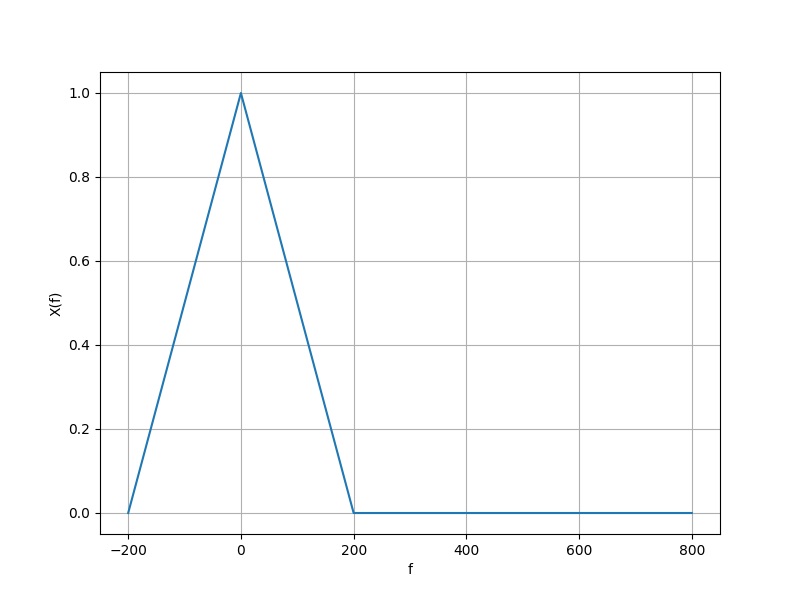
\includegraphics[width=\columnwidth]{2023/BM/33/figs/f1.png}
    \caption{Plot of $X\brak{f}$}
    \label{fig:nikh1}
\end{figure}

\begin{figure}[h!]
    \centering
    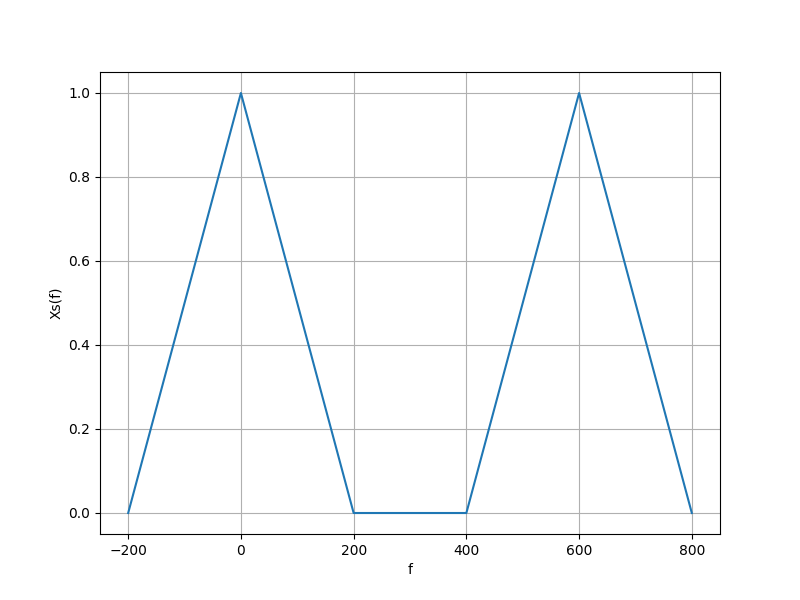
\includegraphics[width=\columnwidth]{2023/BM/33/figs/f2.png}
    \caption{Plot of $X_s\brak{f}$}
    \label{fig:nikh2}
\end{figure}


%\end{document}
